% Chapter Template

\chapter{Motivation and Problem Statement} % Main chapter title

\label{Chapter6}


%-------------------------------------------------------------------------------
%	SECTION 1
\section{Computed Tomography Imaging}
%-------------------------------------------------------------------------------

\ac{ct} imaging is a powerful medical imaging technique that provides detailed
cross-sectional images of a body by combining multiple X-ray projections taken
from different angles. This technique is widely used for diagnostic purposes,
allowing clinicians to visualize internal structures with high spatial
resolution.

The process involves rotating an X-ray source around the patient while
simultaneously capturing X-ray projections on a detector array. Each projection
represents the cumulative attenuation of X-rays as they pass through various
tissues, which is influenced by the density and composition of the materials
they encounter. 

The collected data is then reconstructed into a three-dimensional volume
using sophisticated algorithms, such as filtered backprojection or iterative
reconstruction methods. These algorithms convert the raw projection data into
cross-sectional images, which can be further processed to enhance contrast,
reduce noise and improve overall image quality.

To achieve accurate reconstructions, it is crucial to have precise and high-quality X-ray images. However, one of the most significant challenges in CT imaging is
the presence of scattered radiation, which can lead to artifacts and distortions
in the reconstructed images.

Throughout this thesis, the term \textit{scatter reduction in \ac{ct}} refers to the mitigation of scatter-induced artifacts in the 2D X-ray projection images acquired by the detector array during a CT scan. These projections serve as the input for reconstructing the final 3D volume. Given the complexity of the full reconstruction process, the focus of this work will be limited to analyzing and correcting scatter effects at the level of the 2D projection data. 


%-------------------------------------------------------------------------------
%	SECTION 2
\section{X-ray Imaging and the Challenge of Scatter}
%-------------------------------------------------------------------------------

X-ray \ac{ct} relies on measuring the attenuation of X-ray photons as they
traverse straight-line paths through a phantom. These trajectories typically
extend from an X-ray source $S$ to a detector element $\mathcal{D}_j$, forming
the path:

$$l=\overrightarrow{S\mathcal{D}_j}$$

Under idealized conditions, the attenuation process is goverend by the
Lambert-Beer law, which describes an exponential decay in intensity as the beam
interacts with the material. As stated in \cite[Chap.
7]{medicalImagingSystemsIntro2019:} ,this relationship is given by

\begin{equation}
    \label{eq:lambert_beer_law}
     I = \int_0^{E_\text{max}}{I_0(E)\cdot \exp\bigg(-\int_{S}^{\mathcal{D}_j}{\mu(x,E)dx}\bigg)} dE
\end{equation}
where $I_0(E)$ denotes the incident intensity of X-rays with energy $E$ at
source $S$. Further $\mu(x,E)$ represents the linear attenuation coefficient of
a photon at any spatial location $x$ along the path $l$ with energy $E$. The
resulting intensity $I$ is measured at the detector element $\mathcal{D}_j$.

Although exponential attenuation along straight-line paths is the idealized
model for X-ray imaging, this assumption is systematically violated in practice.
As X-rays traverse the scanned object, many photons undergo scattering
interactions - such as Compton or Rayleigh scattering - which alter their
trajectories. Despite deviating from the primary path, these scattered photons
may still reach the detector, adding unintended signal components. As a result,
the measured intensities no longer represent pure line integrals of the
attenuation map. This discrepancy introduces nonlinear errors and visible
artifacts in the reconstructed image, ultimately degrading both visual quality
and quantitative accuracy.

Scattered radiation is a major source of image artifacts - such as cupping and
streaks - and reduces both spatial and contrast resolution. These effects not
only degrade visual image quality but also compromise the accuracy of
quantitative measurements, such as Hounsfield units $\mu_*$ \cite[Chap.
8]{medicalImagingSystemsIntro2019:}, which are used for clinical interpretation
such as tissue characterization. Hounsfield units are representing a
normalized attenuation to the attenuation of water.

$$\mu_* = \left(\frac{\mu}{\mu_{\text{water}}} -1\right) \cdot 1000$$

The impact of scatter becomes especially pronounced in modern CT systems using
high-energy X-rays or large-area flat-panel detectors, where scatter may
dominate the measured signal. As such, accurate modeling and correction of
scatter is essential for achieving high-fidelity CT images, particularly in
clinical applications where precision and reliability are paramount
\citep{medicalImagingSystemsIntro2019:}.


%-------------------------------------------------------------------------------
%	SECTION 3
\section{Scatter Correction Methods for X-ray Imaging}
%-------------------------------------------------------------------------------

\subsection{Overview of Scatter Correction Techniques}

In \ac{ct}, scattered photons are a major source of image artifacts and
quantitative inaccuracies. To mitigate these effects, a range of computational
scatter correction methods has been developed. These approaches can be broadly
classified into the following categories:

\begin{itemize}
    \item \textbf{Empirical and Analytical Methods:} \\
        These include techniques such as primary modulation, convolution-based
        correction and energy windowing. Scatter is typically estimated using
        simplified models or empirical kernels, often assuming a smooth
        background distribution and then subtracted from the measured signal.
        While computationally efficient, these methods rely on assumptions
        regarding the spatial and energy distribution of scattered photons. As a
        result, they may fail to accurately model complex scatter phenomena in
        heterogeneous anatomical structures.
    \item \textbf{Physics-Based Models:} \\
        These methods aim to provide a more accurate representation of the
        underlying photon transport physics, including scattering phenomena.
        Among them, Monte Carlo (MC) simulation is regarded as the most rigorous
        and comprehensive technique due to its ability to statistically model
        complex photon interactions without relying on simplifying assumptions.
        In such models, primary and scattered photon contributions are simulated
        separately, allowing the estimated scatter signal to be subtracted from
        measured data in order to restore image fidelity.
    \item \textcolor{green}{TODO: AI Method from Josha Maier?}
\end{itemize}

In \citeyear{mcffd2011} \citeauthor{mcffd2011} \cite{mcffd2011} already
demonstrated promising results using the computationally expensive \ac{mc}
simulation of the \ac{ct} of a cylinder phantom with two bone inserts. The
results show significant improvements in the image quality as demonstrated by
\citeauthor{mcffd2011} in Figure~\ref{fig:scatter_correction_comparison}.

\captionsetup{justification=justified,singlelinecheck=false}
\begin{figure}[!h]
    \centering
    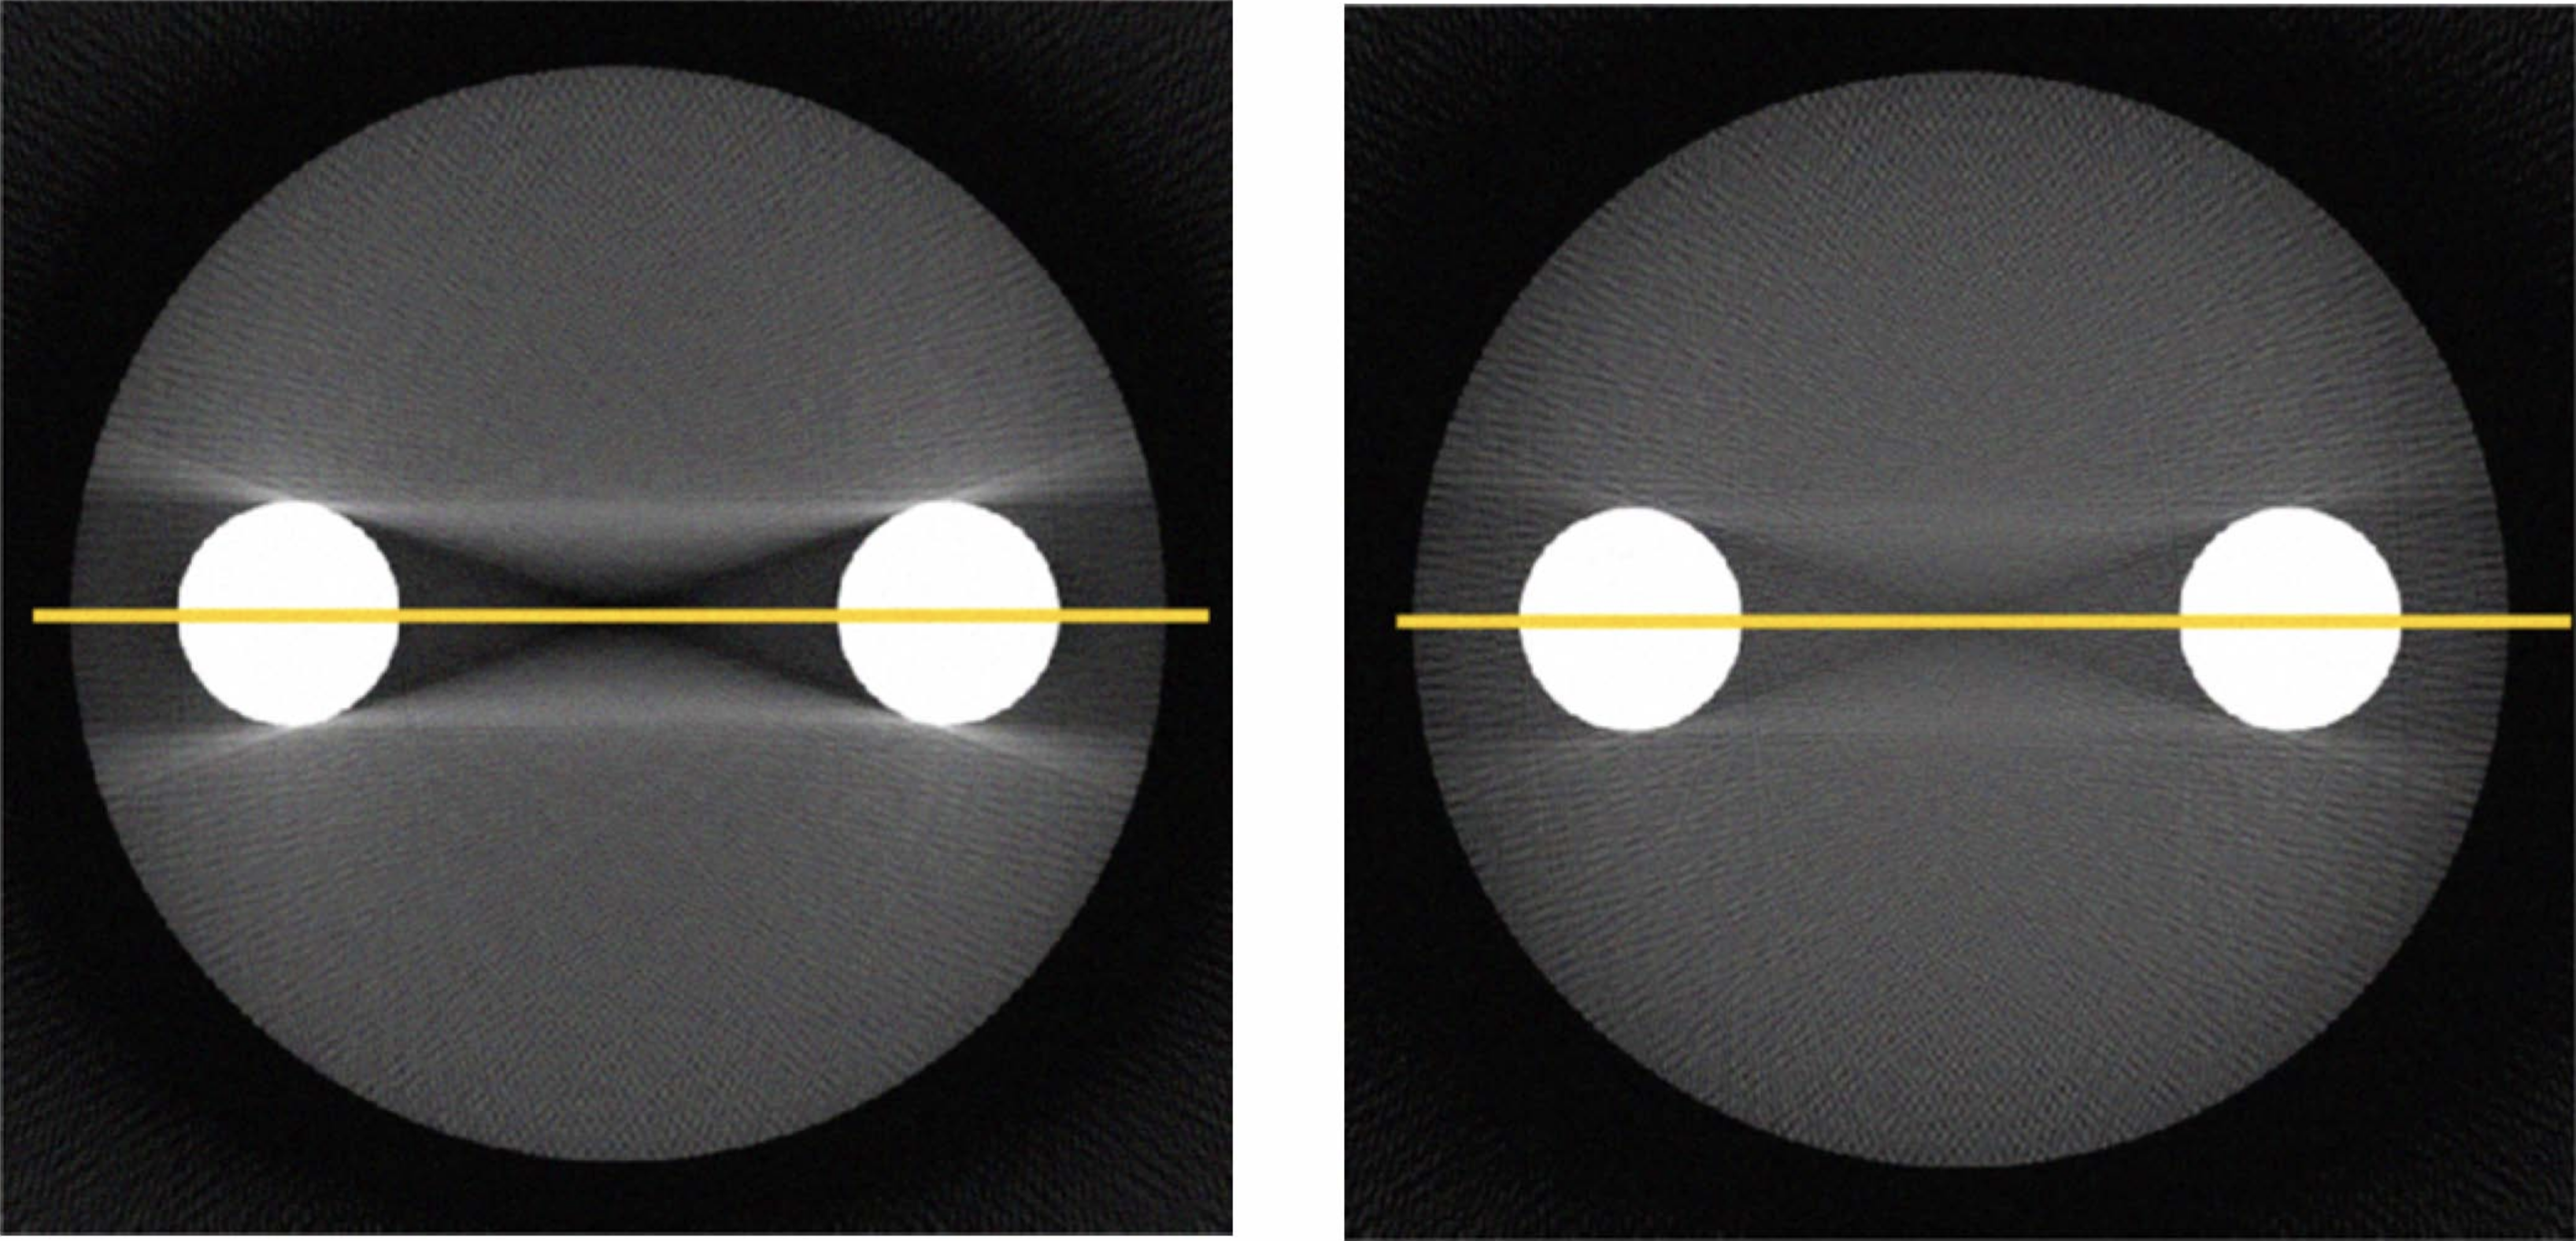
\includegraphics[width=0.8\textwidth]{Figures/mcffd.png}
    \caption{\ac{cbct} of a 70 mm soft-tissue cylinder with two bone inserts.
    Left: Image after scatter correction using the gMCFFD method ($5e6$
    photons), showing improved uniformity and quantitative accuracy. Right:
    Image without correction, exhibiting typical cupping and streak artifacts.
    (from \cite{mcffd2011})}
    \label{fig:scatter_correction_comparison}
\end{figure}

\subsection{Monte Carlo Simulation}

The \ac{mc} simulation is a powerful computational technique that follows
phyics-based principles to model the transport of photons through matter. It is
widely recognized as the gold standard for scatter correction in CT and related
imaging modalities. This status is attributed to several key factors:

\begin{itemize}
    \item \textbf{Physical Accuracy:} \\
    \ac{mc} methods simulate the stochastic nature of photon interactions
    (including Compton and Rayleigh scattering, photoelectric absorption and
    multiple scattering events) based on fundamental physical cross-sections and
    material properties.

    \item \textbf{Comprehensive Modeling:} \\
    Unlike analytical or empirical methods, \ac{mc} simulation can account for
    complex geometries, heterogeneous materials and realistic X-ray spectra,
    providing highly accurate estimates of the scatter signal.

    \item \textbf{Validation Benchmark:} \\
    Due to their accuracy, \ac{mc}-based scatter estimates are routinely used as
    reference standards for validating and benchmarking faster, approximate
    correction methods.
\end{itemize}


% ------------------------------------------------------------------------------
%	SECTION 4
\section{High-Level Overview of the Monte Carlo Simulation}
%-------------------------------------------------------------------------------

Monte Carlo simulation of photon transport for scatter correction involves the
following key steps \cite{mcffd2011}:

\begin{enumerate}
    \item \textbf{Photon Emission:} \\
        Photons are emitted from a virtual X-ray source, with energies sampled
        from the source spectrum.
    \item \textbf{Photon Tracking:} \\
        Each photon is tracked as it propagates through the object. At each
        step, the probability of interaction (scattering or absorption) is
        determined by the local material properties and cross-sections.
    \item \textbf{Interaction Sampling:} \\
        When an interaction occurs, the type (e.g., Compton, Rayleigh or
        Absorption) and the resulting change in photon direction and energy are
        sampled from the relevant probability distributions.
    \item \textbf{Detection:} \\
        Photons that reach the detector (either unscattered or after one or more
        scatter events) are recorded. The simulation keeps track of both primary
        and scattered photons, allowing for the estimation of the scatter
        contribution to each detector element.
    \item \textbf{Statistical Averaging:} \\
        By simulating a large number of photons the method builds up a
        statistical robust estimate of the scatter distribution. The accuracy of
        the result increases with the number of simulated photons and eventually
        converges to a stable intensity distribution.
\end{enumerate}

The schematic flow of the Monte Carlo simulation process is illustrated in
Figure~\ref{fig:photon-transport-pseudocode}.

\begin{figure}[!h]
\centering
\begin{tcolorbox}[colback=white!95!gray, colframe=black!60, width=0.9 \textwidth, title=Monte Carlo Photon Transport Algorithm, fonttitle=\bfseries]
\begin{itemize}[leftmargin=1.5em]
    \item \textbf{Initialization:} Define geometry, materials and source
    spectrum.
    \item \textbf{Loop over photons:}
    \begin{itemize}
        \item Sample step size to next interaction.
        \item Move photon; check for boundary crossing.
        \item Sample interaction type; update direction/energy.
        \item If photon reaches detector, record event.
        \item If photon is absorbed or leaves the system, terminate.
    \end{itemize}
    \item \textbf{Aggregate results:} Compute scatter and primary distributions.
\end{itemize}
\end{tcolorbox}
\caption{Pseudocode for photon transport simulation in Monte Carlo scatter modeling.}
\label{fig:photon-transport-pseudocode}
\end{figure}


%-------------------------------------------------------------------------------%	SECTION 5
\section{Monte Carlo Methods: Benefits \& Drawbacks}
%-------------------------------------------------------------------------------
\textcolor{green}{QMC still does not appear in the caption}

Monte Carlo (MC) simulations are widely regarded as the gold standard for
scatter correction in computed tomography due to their ability to model
photon-matter interactions from first principles. These simulations faithfully
reproduce all relevant physical scattering phenomena - including Compton and
Rayleigh scattering - and can accommodate arbitrarily complex object geometries
and heterogeneous material compositions. Owing to this high level of physical
realism, MC-based methods yield highly accurate scatter estimates and are
therefore commonly used as a reference benchmark for evaluating and validating
alternative correction approaches.

However, the high accuracy of Monte Carlo simulations comes at the cost of
substantial computational demand. Achieving low-noise scatter estimates requires
simulating a large number of photon histories to ensure statistical convergence.
As a result, the runtime scales with the desired level of accuracy and can span
from several minutes to multiple hours or even days, depending on the complexity
of the problem and the available computational resources. This computational
burden poses a major practical limitation, particularly in scenarios involving
large datasets or iterative reconstruction workflows.

In response to the computational burden of slow converging traditional Monte
Carlo methods, recent research has focused on approaches to accelerate this type
of precisely correct photon transport simulations. Among these, the application
\ac{qmc} methods has gained increasing attention. By replacing random sampling
with deterministic low-discrepancy sequences, QMC techniques achieve
significantly faster convergence while maintaining comparable accuracy.
Contemporary QMC-based scatter correction algorithms have demonstrated runtime
reductions of one to two orders of magnitude, thereby enabling high-fidelity
simulations even in time-sensitive or resource-constrained settings
\cite{qmcXray2023}.
